\section{Bangkok}

12 juin 2008

\begin{multicols}{2}

Alors alors... Je vous ai laissés à Hua Hin, petite ville en passe de devenir une grosse station balnéaire à 3 heures de bus de Bangkok. Je n'ai pas énormément de choses à vous dire à propos de cette ville, si ce n'est que le patron de la guest house "All Nations" est Anglais, et qu'il est fan de tennis. Nous avons regardé Roland Garros ensembles. Je suis resté 3 nuits a Hua Hin puis j'ai pris le bus pour Bangkok.

Pout tout vous dire j'ai hésité à appeler cet article "Marchés a Bangkok", ou "Marcher à Bangkok". C'est donc tout logiquement que j'ai choisi un troisième titre.

Bangkok... très grande ville, bien sympa à découvrir. On peut trouver tout ce que l'on veut il suffit de bien chercher. Cependant si vous voulez une montre Rolex ou une écharpe Gucci, le premier petit marchand ambulant fera l'affaire... Bien sûr n'allez pas lui demander un reçu ou un certificat de conformité.

J'ai été très bien accueilli par Cécile, une amie de mes parents qui est prof de maths à Bangkok, puis Célia, sa fille, nous a rejoint, elle rentrait d'un stage de 3 mois au Viêtnam. Autant vous dire qu'on a pas arrété de parler de voyages.

La visite de la ville a commencé en prenant un bateau sur un des klongs, les klongs sont des canaux, pas toujours accueillants par leur odeur, mais permettant de voir un coté non touristique. Une petite photo pour se mettre dans l'ambience, et la video après.

\smallbreak
\hspace*{-0.65cm}
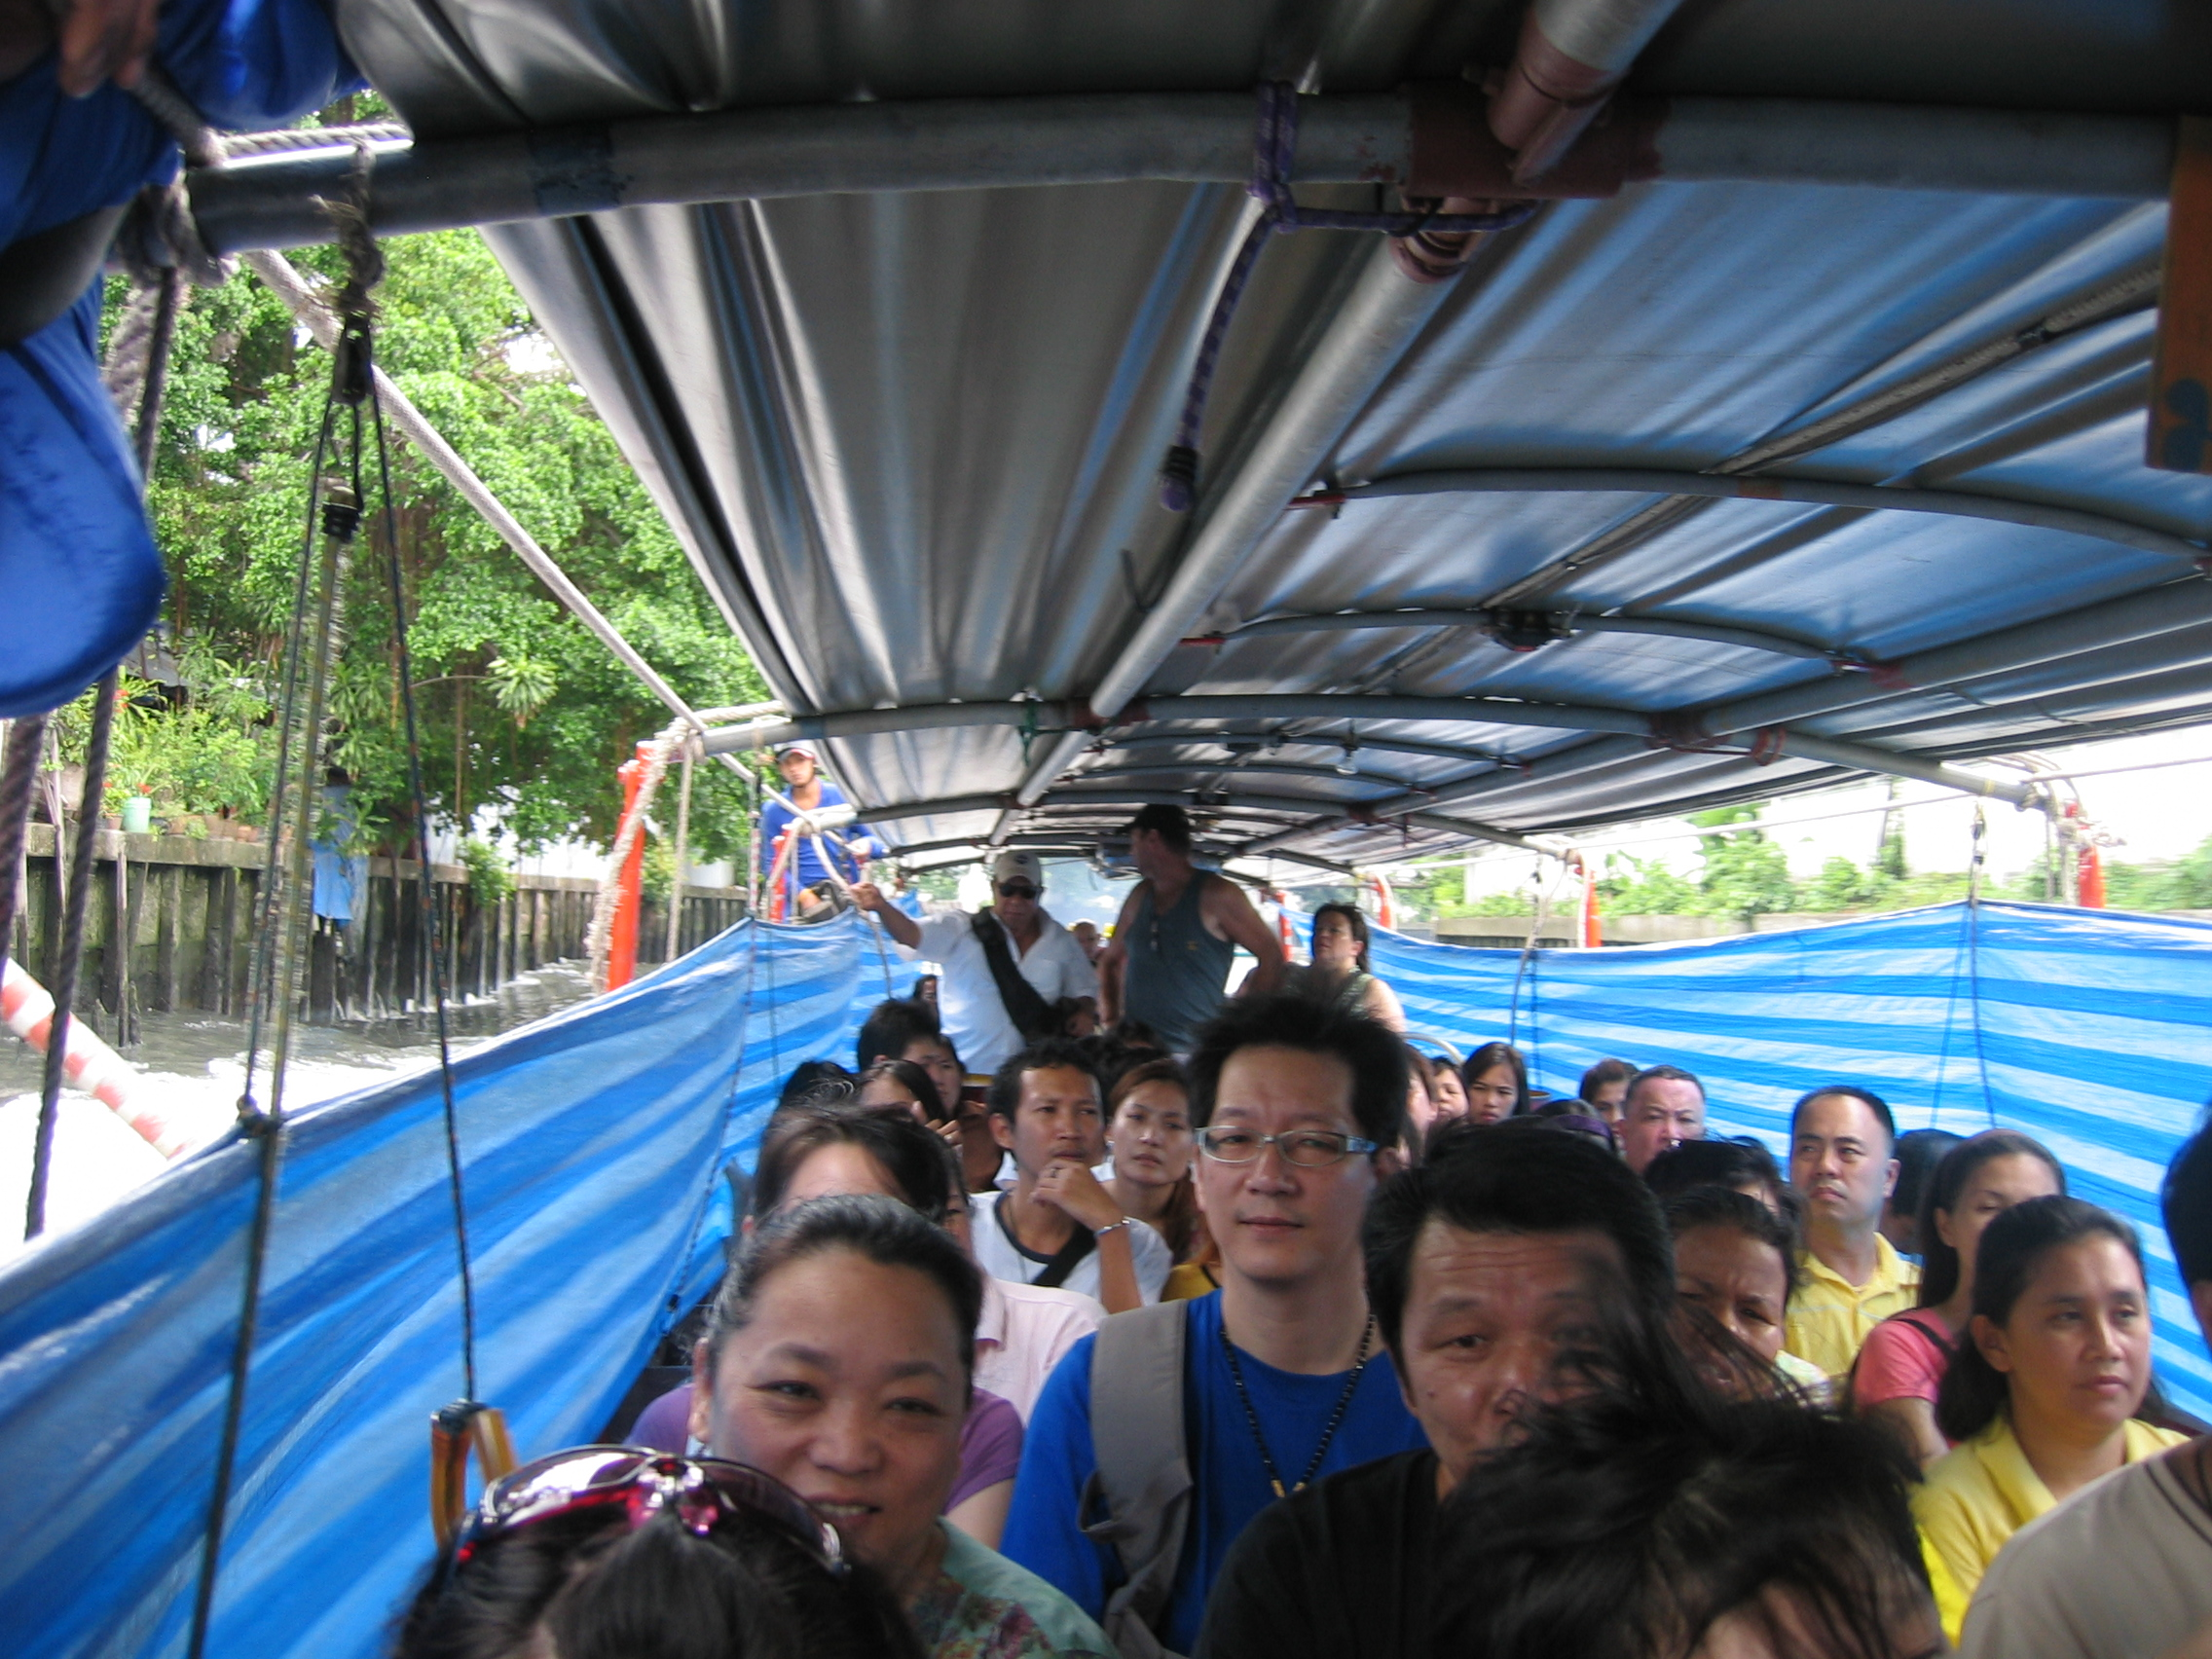
\includegraphics[width=5cm]{articles/Bangkok/1345.jpg}
%Bateau sur un Klong.
\smallbreak

%<div><object width="640" height="505"><param name="movie" value="http://www.dailymotion.com/swf/x5n17d&related=1"></param><param name="allowFullScreen" value="true"></param><param name="allowScriptAccess" value="always"></param><embed src="http://www.dailymotion.com/swf/x5n17d&related=1" type="application/x-shockwave-flash" width="640" height="505" allowFullScreen="true" allowScriptAccess="always"></embed></object></div>

Puis je suis allé voir le Jim Thomson museum. Il s'agit d'un petit musée regroupant la collection d'art d'un certain Jim Thomson comme vous l'aurez compris. J'ai surtout apprécié ça pour l'architecture des petites maisons en bois, on ne s'attend pas à voir ça en plein centre de Bangkok.

\smallbreak
\hspace*{-0.65cm}
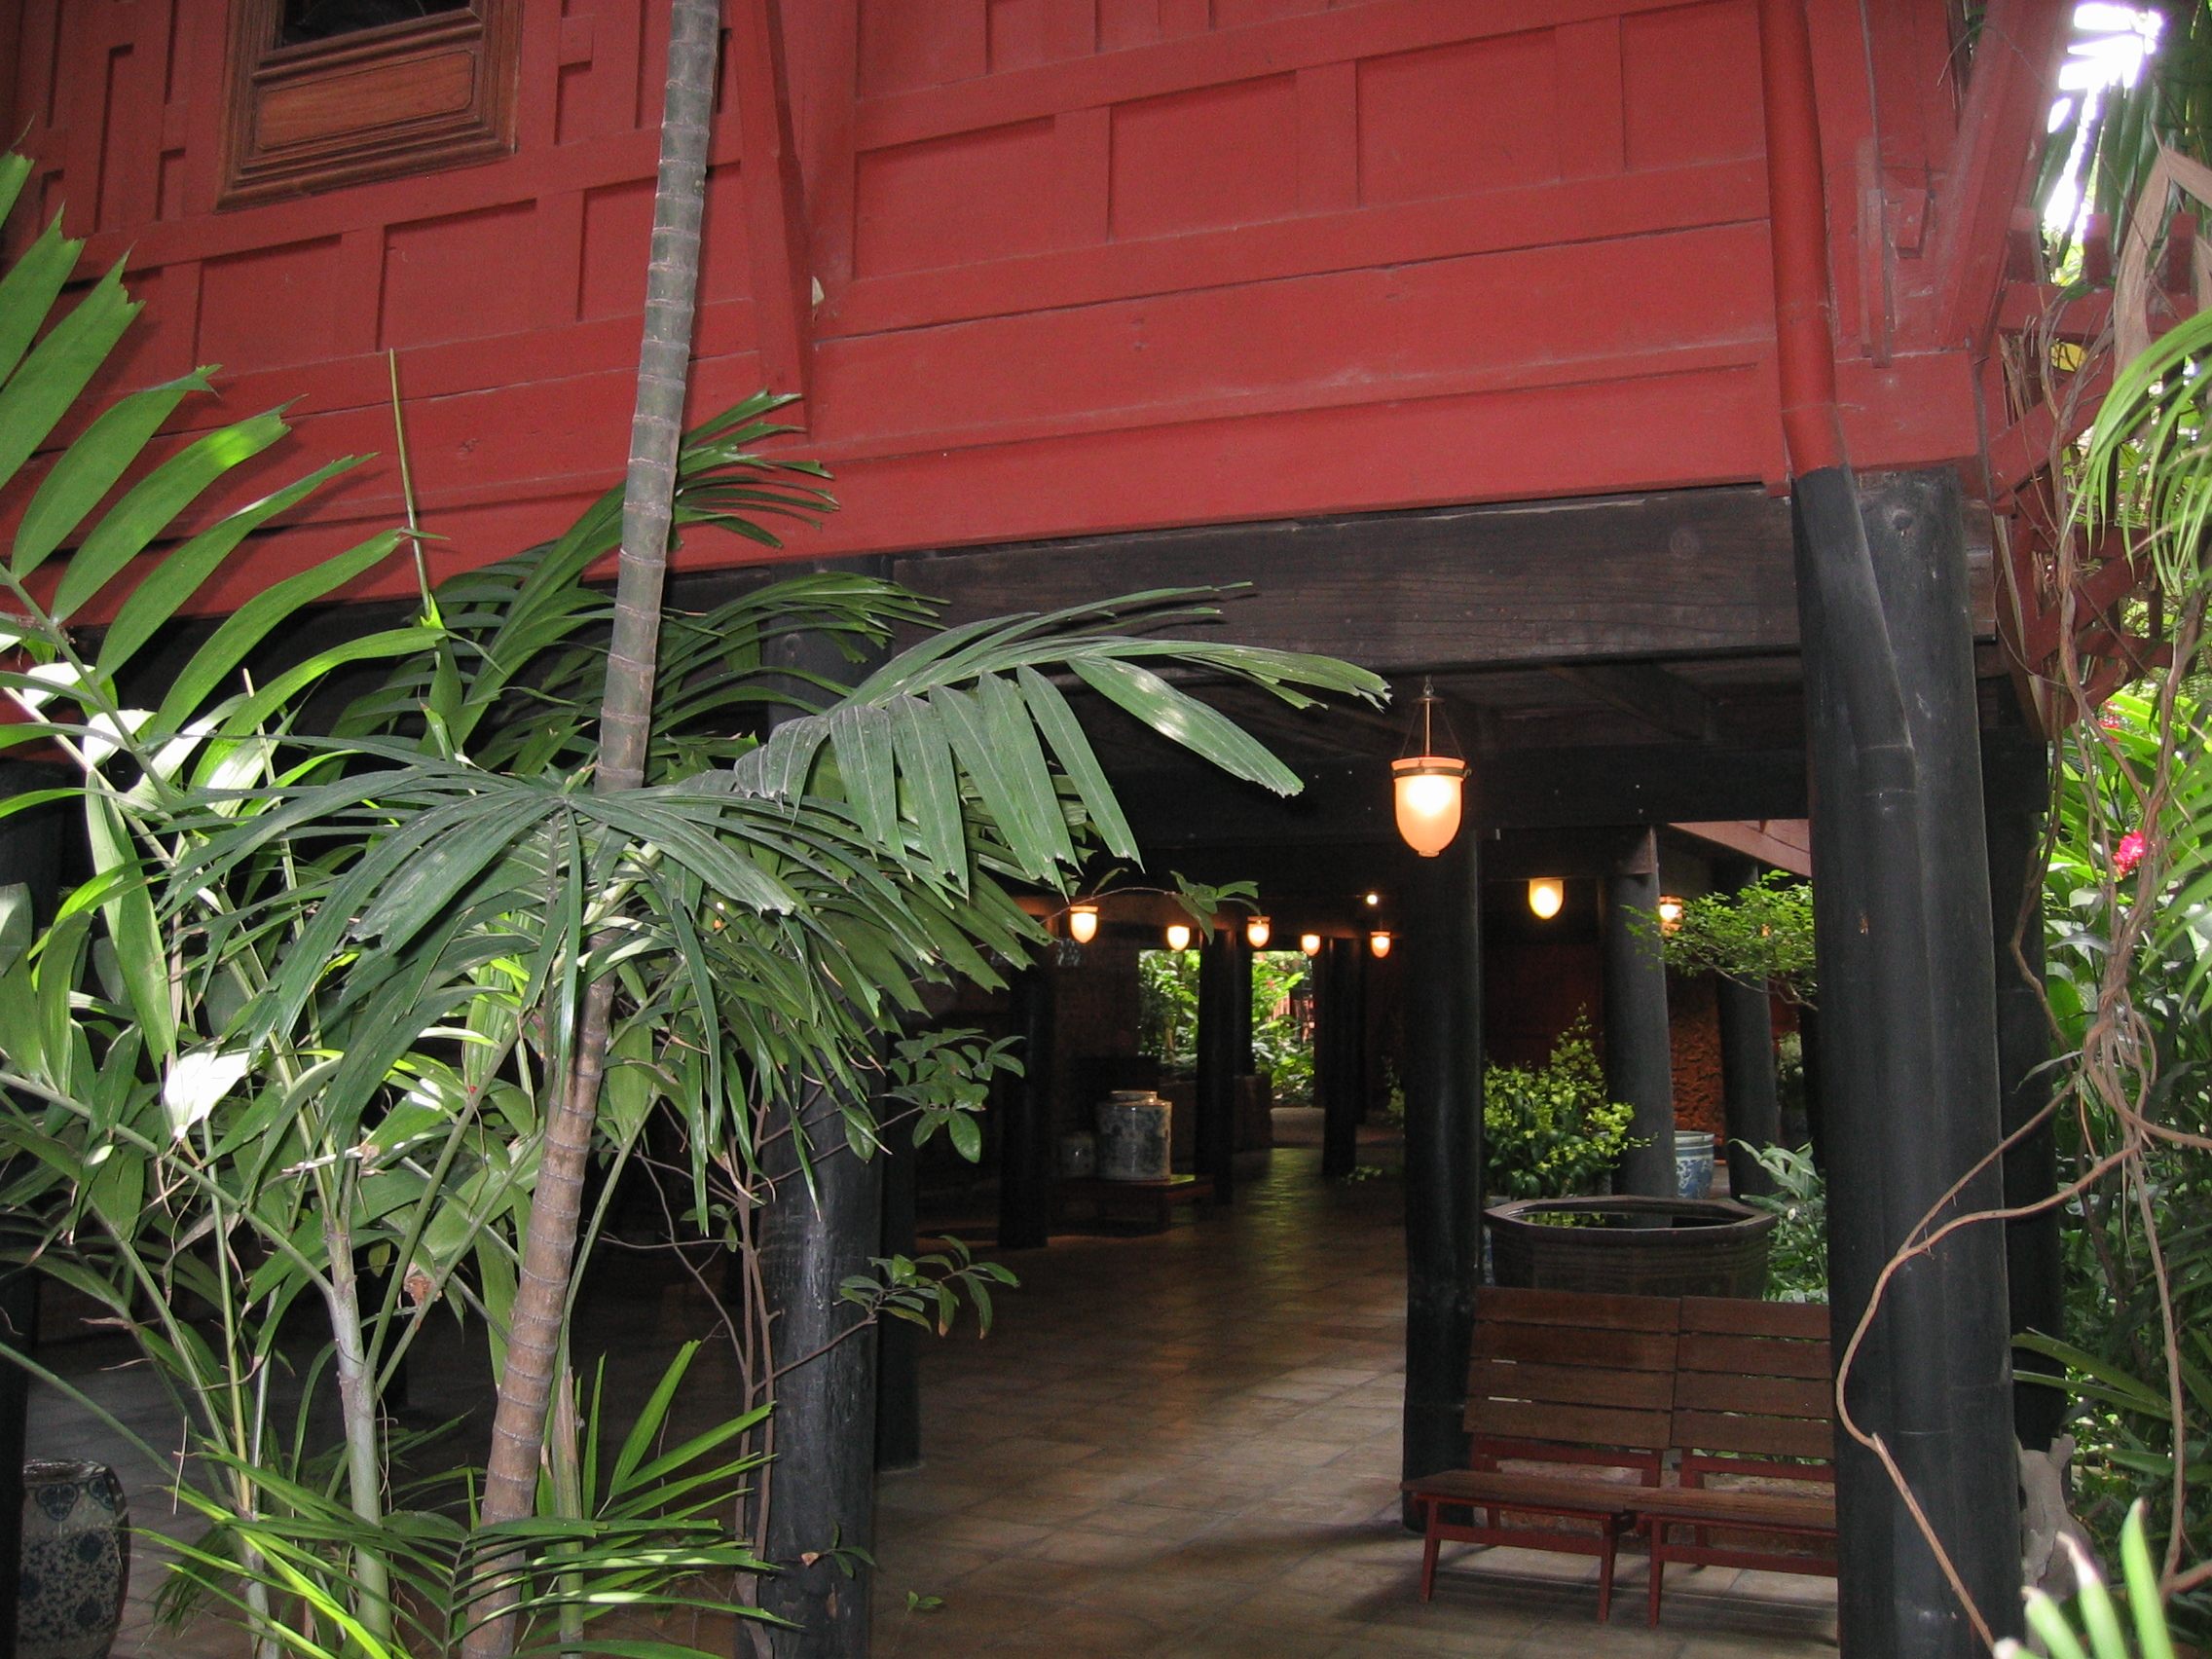
\includegraphics[width=5cm]{articles/Bangkok/1338.jpg}
%Une Pagode du Thomson Museum.
\smallbreak

Puis je me suis balladé dans la ville, je suis resté en tout un peu plus de 4 jours à Bangkok. Les Thaïlandais adorent leur roi, et ils le montrent. Le lundi est le jour du roi et il est impressionnant de voir le nombre de Thaïs qui s'habillent en jaune (sa couleur) ce jour là. Ils adorent aussi montrer leur drapeau accompagné du drapeau du roi (symbole royal sur fond jaune). Voici une photo d'un batiment.

\smallbreak
\hspace*{-0.65cm}
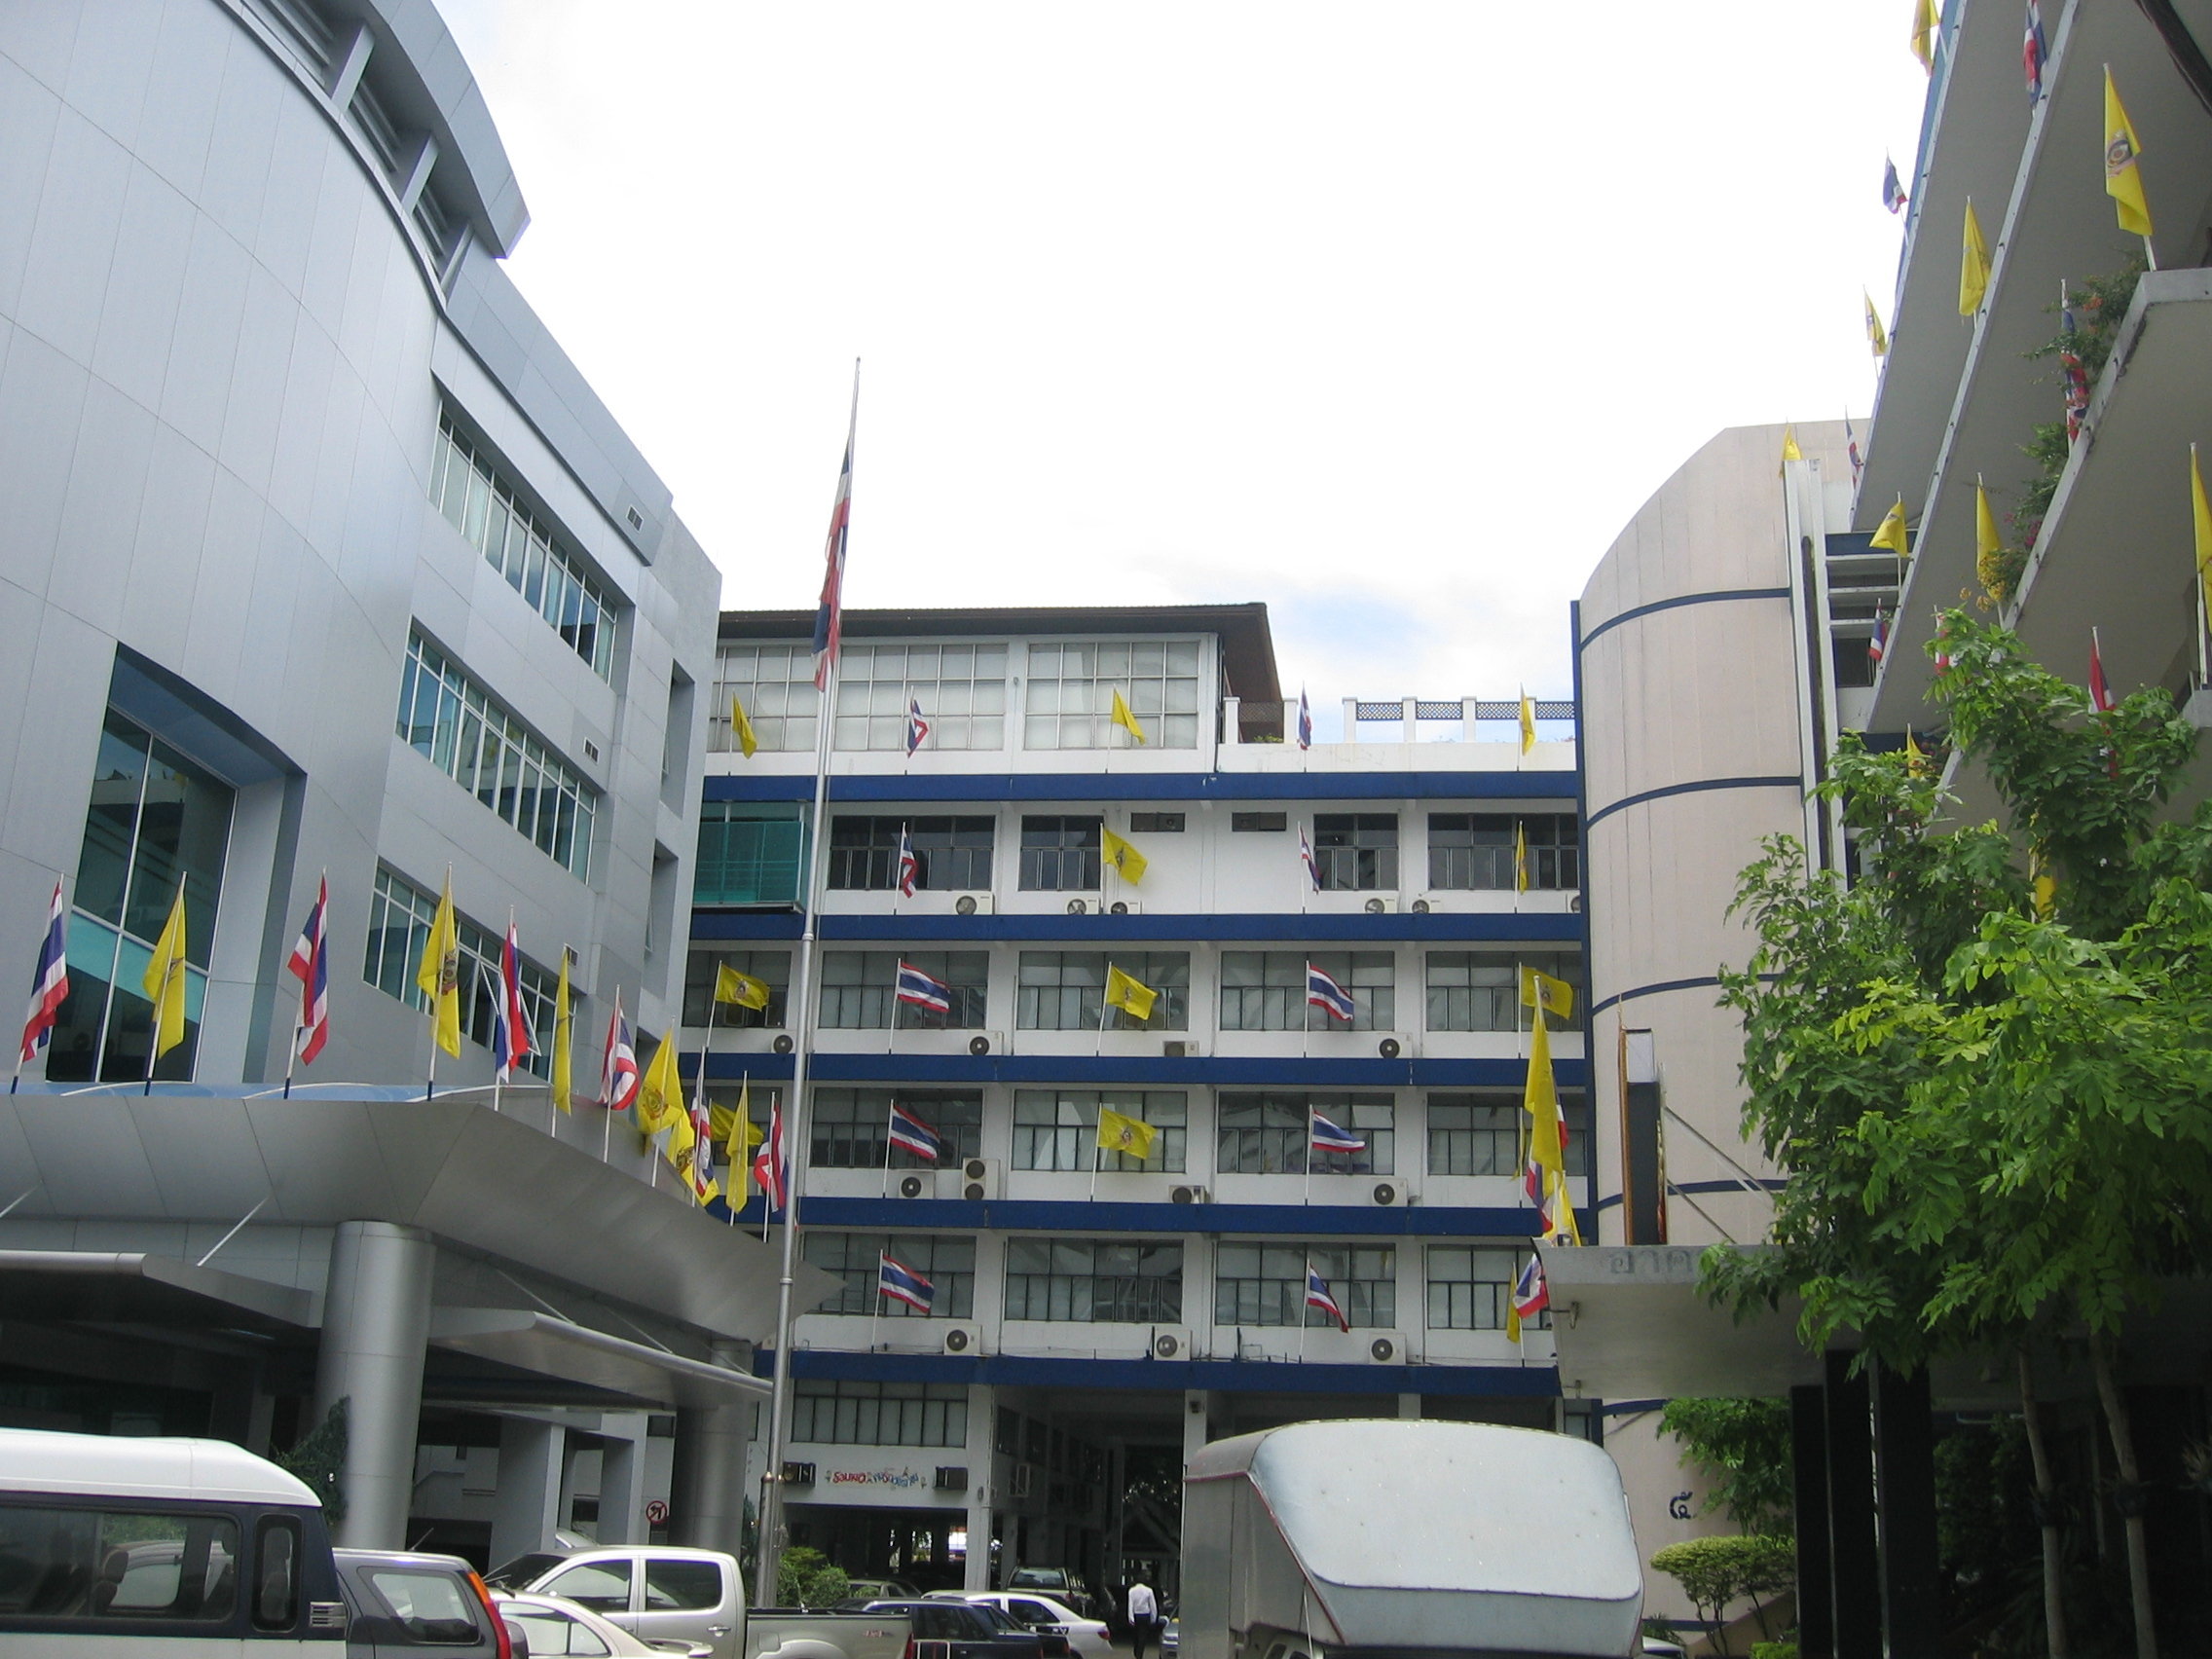
\includegraphics[width=5cm]{articles/Bangkok/1395.jpg}
%Un bâtiment dans Bangkok, avec pleins de drapeaux.
\smallbreak

Comme j'aime bien le bateau (vous le saviez?), je n'ai pas pu m'enpêcher de naviguer sur la Chao Praya, fleuve qui coule du côté Ouest de Bangkok, et c'est l'occasion de vous présenter des bonzes. Un bonze est un prêtre ou moine bouddhiste, très respecté de tous. J'ai fait attention à ne pas les faire tomber dans l'eau, ça aurait fait mauvais genre de couler un bonze dans la rivière (amis des mauvais jeux de mots, bonjour).

\smallbreak
\hspace*{-0.65cm}
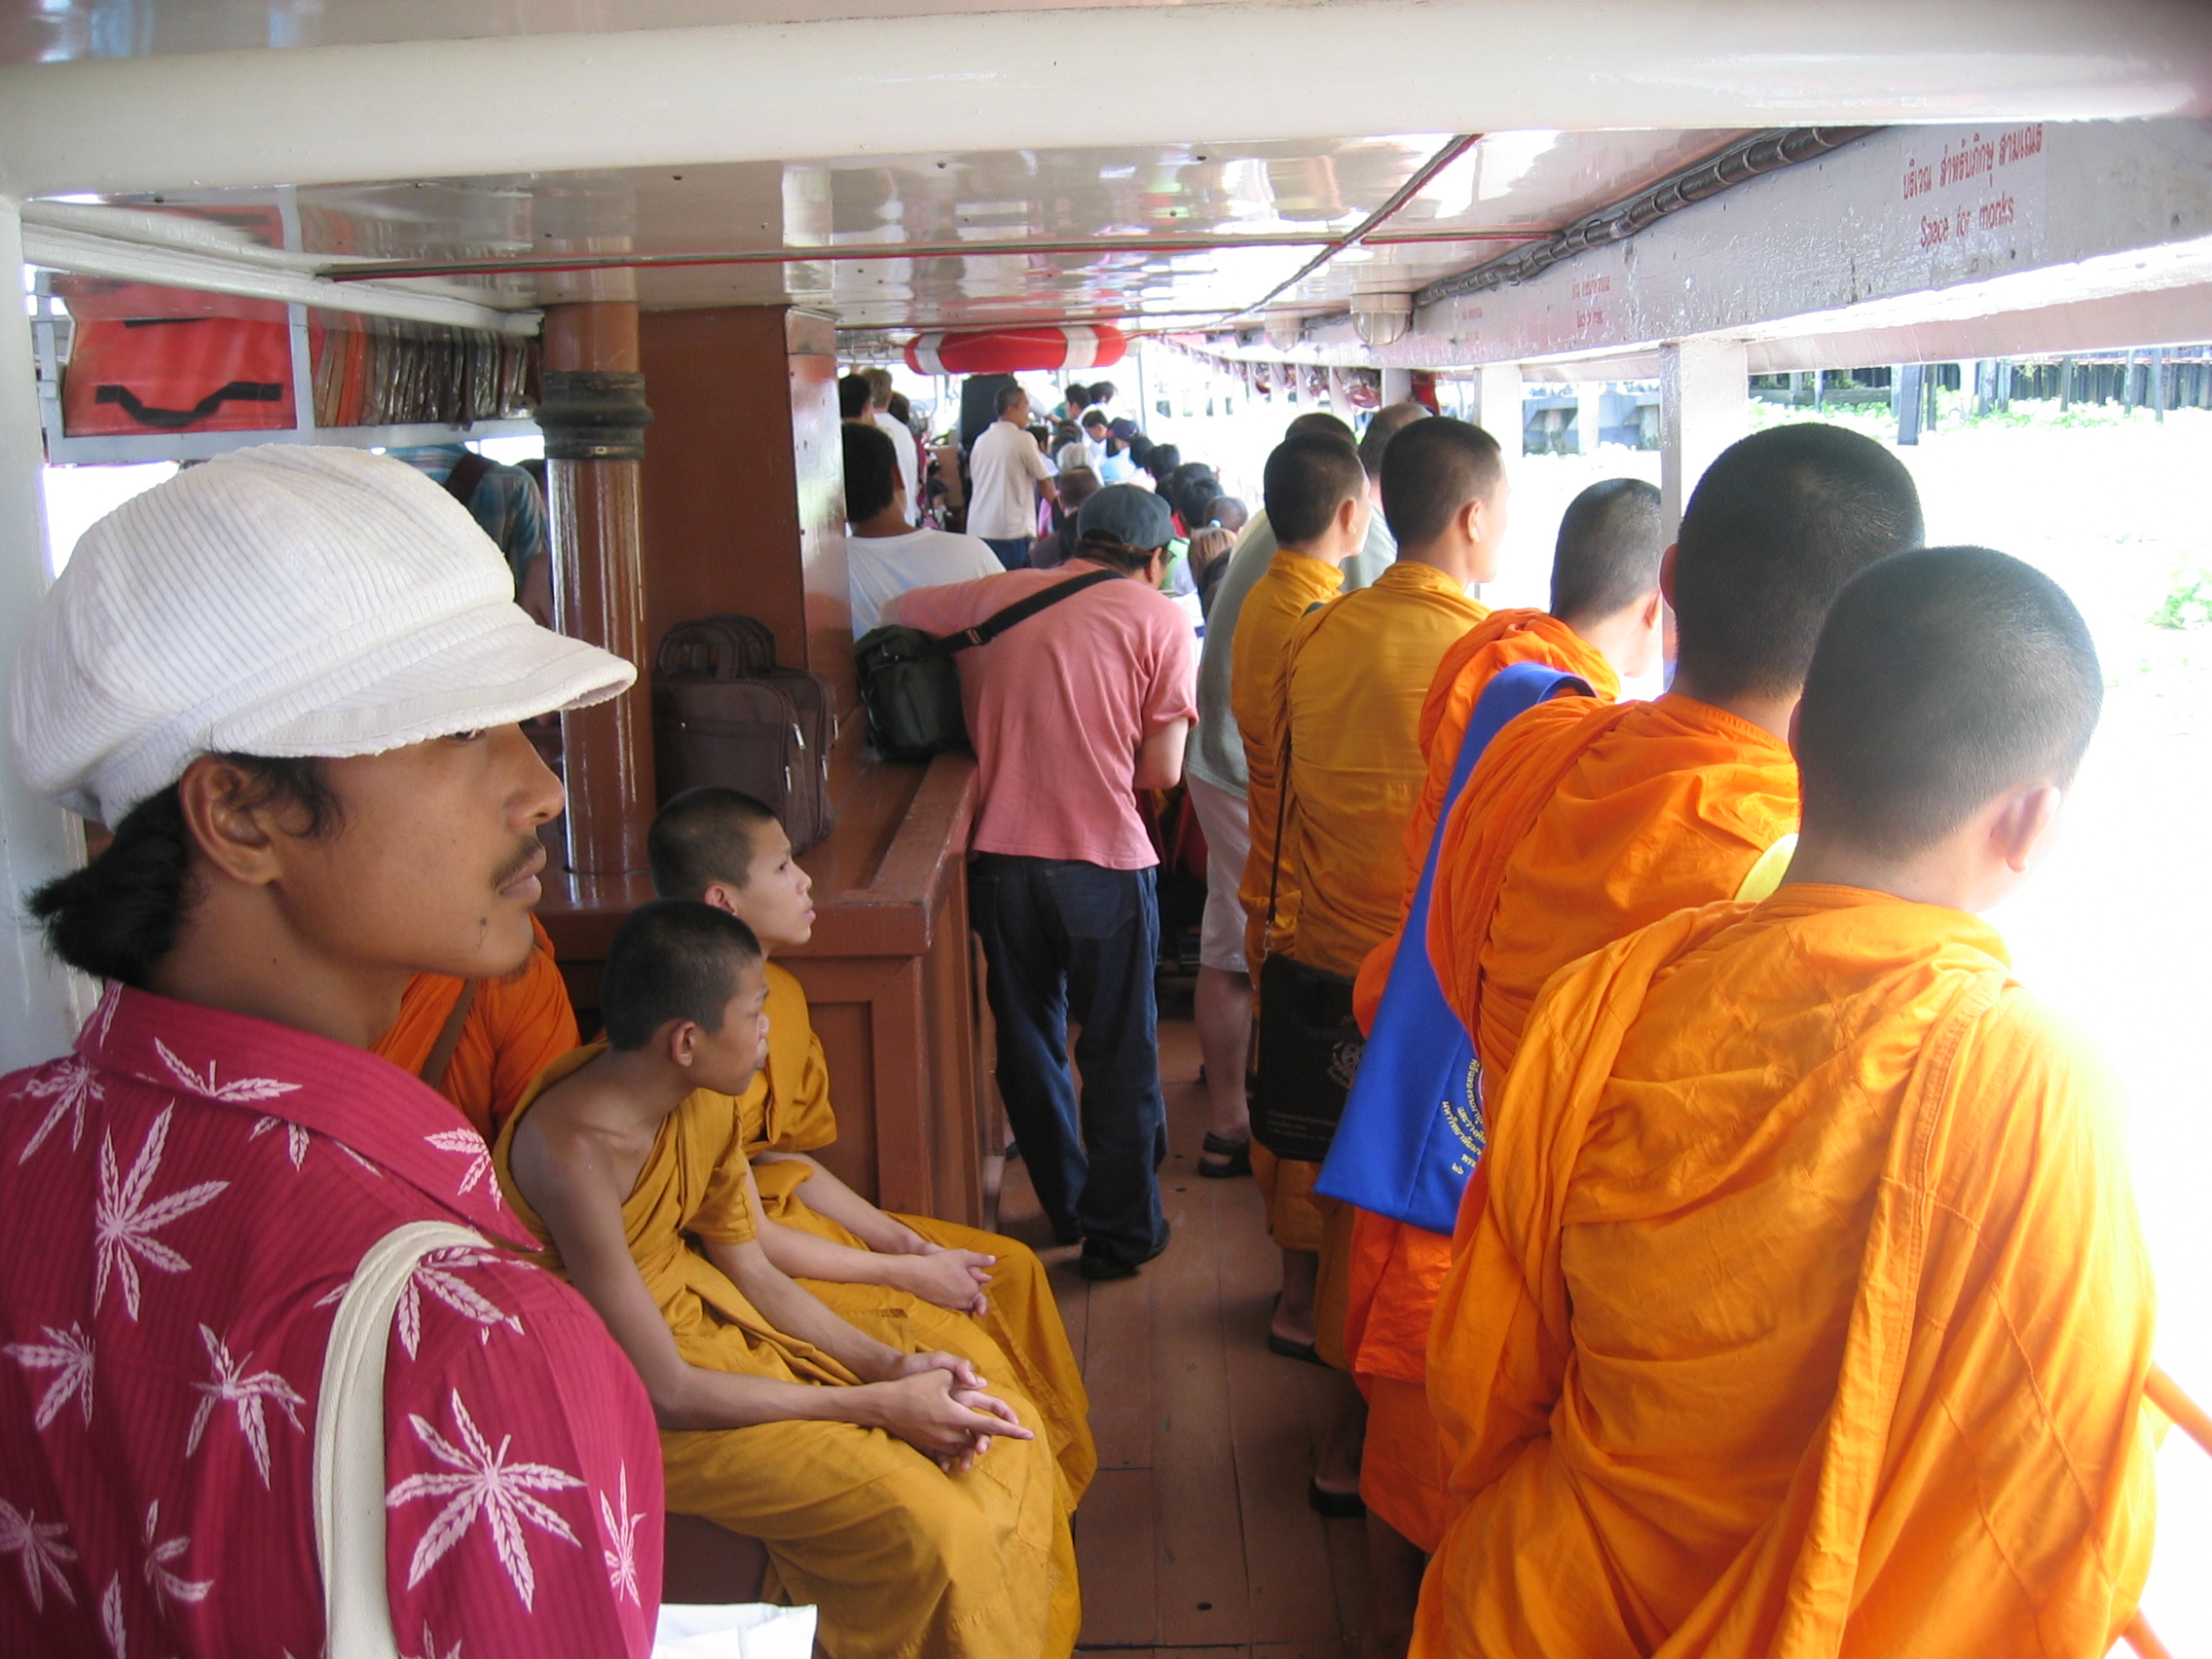
\includegraphics[width=5cm]{articles/Bangkok/1396.jpg}
%Les bonzes sur la Chao Praya.
\smallbreak

Un truc que j'adore maintenant, c'est visiter les marchés. Ici on voit tout, du plus propre (quoique...) au plus sale, mais tout le monde achète et finalement tout se passe bien. En fait c'est nous qui avons un sens du propre trop développé je pense. Cela dit la majorité des stands sont de très bonne qualité, il faut juste fermer les yeux quand on passe devant certains stands de poisson ou de viande.

\smallbreak
\hspace*{-0.65cm}
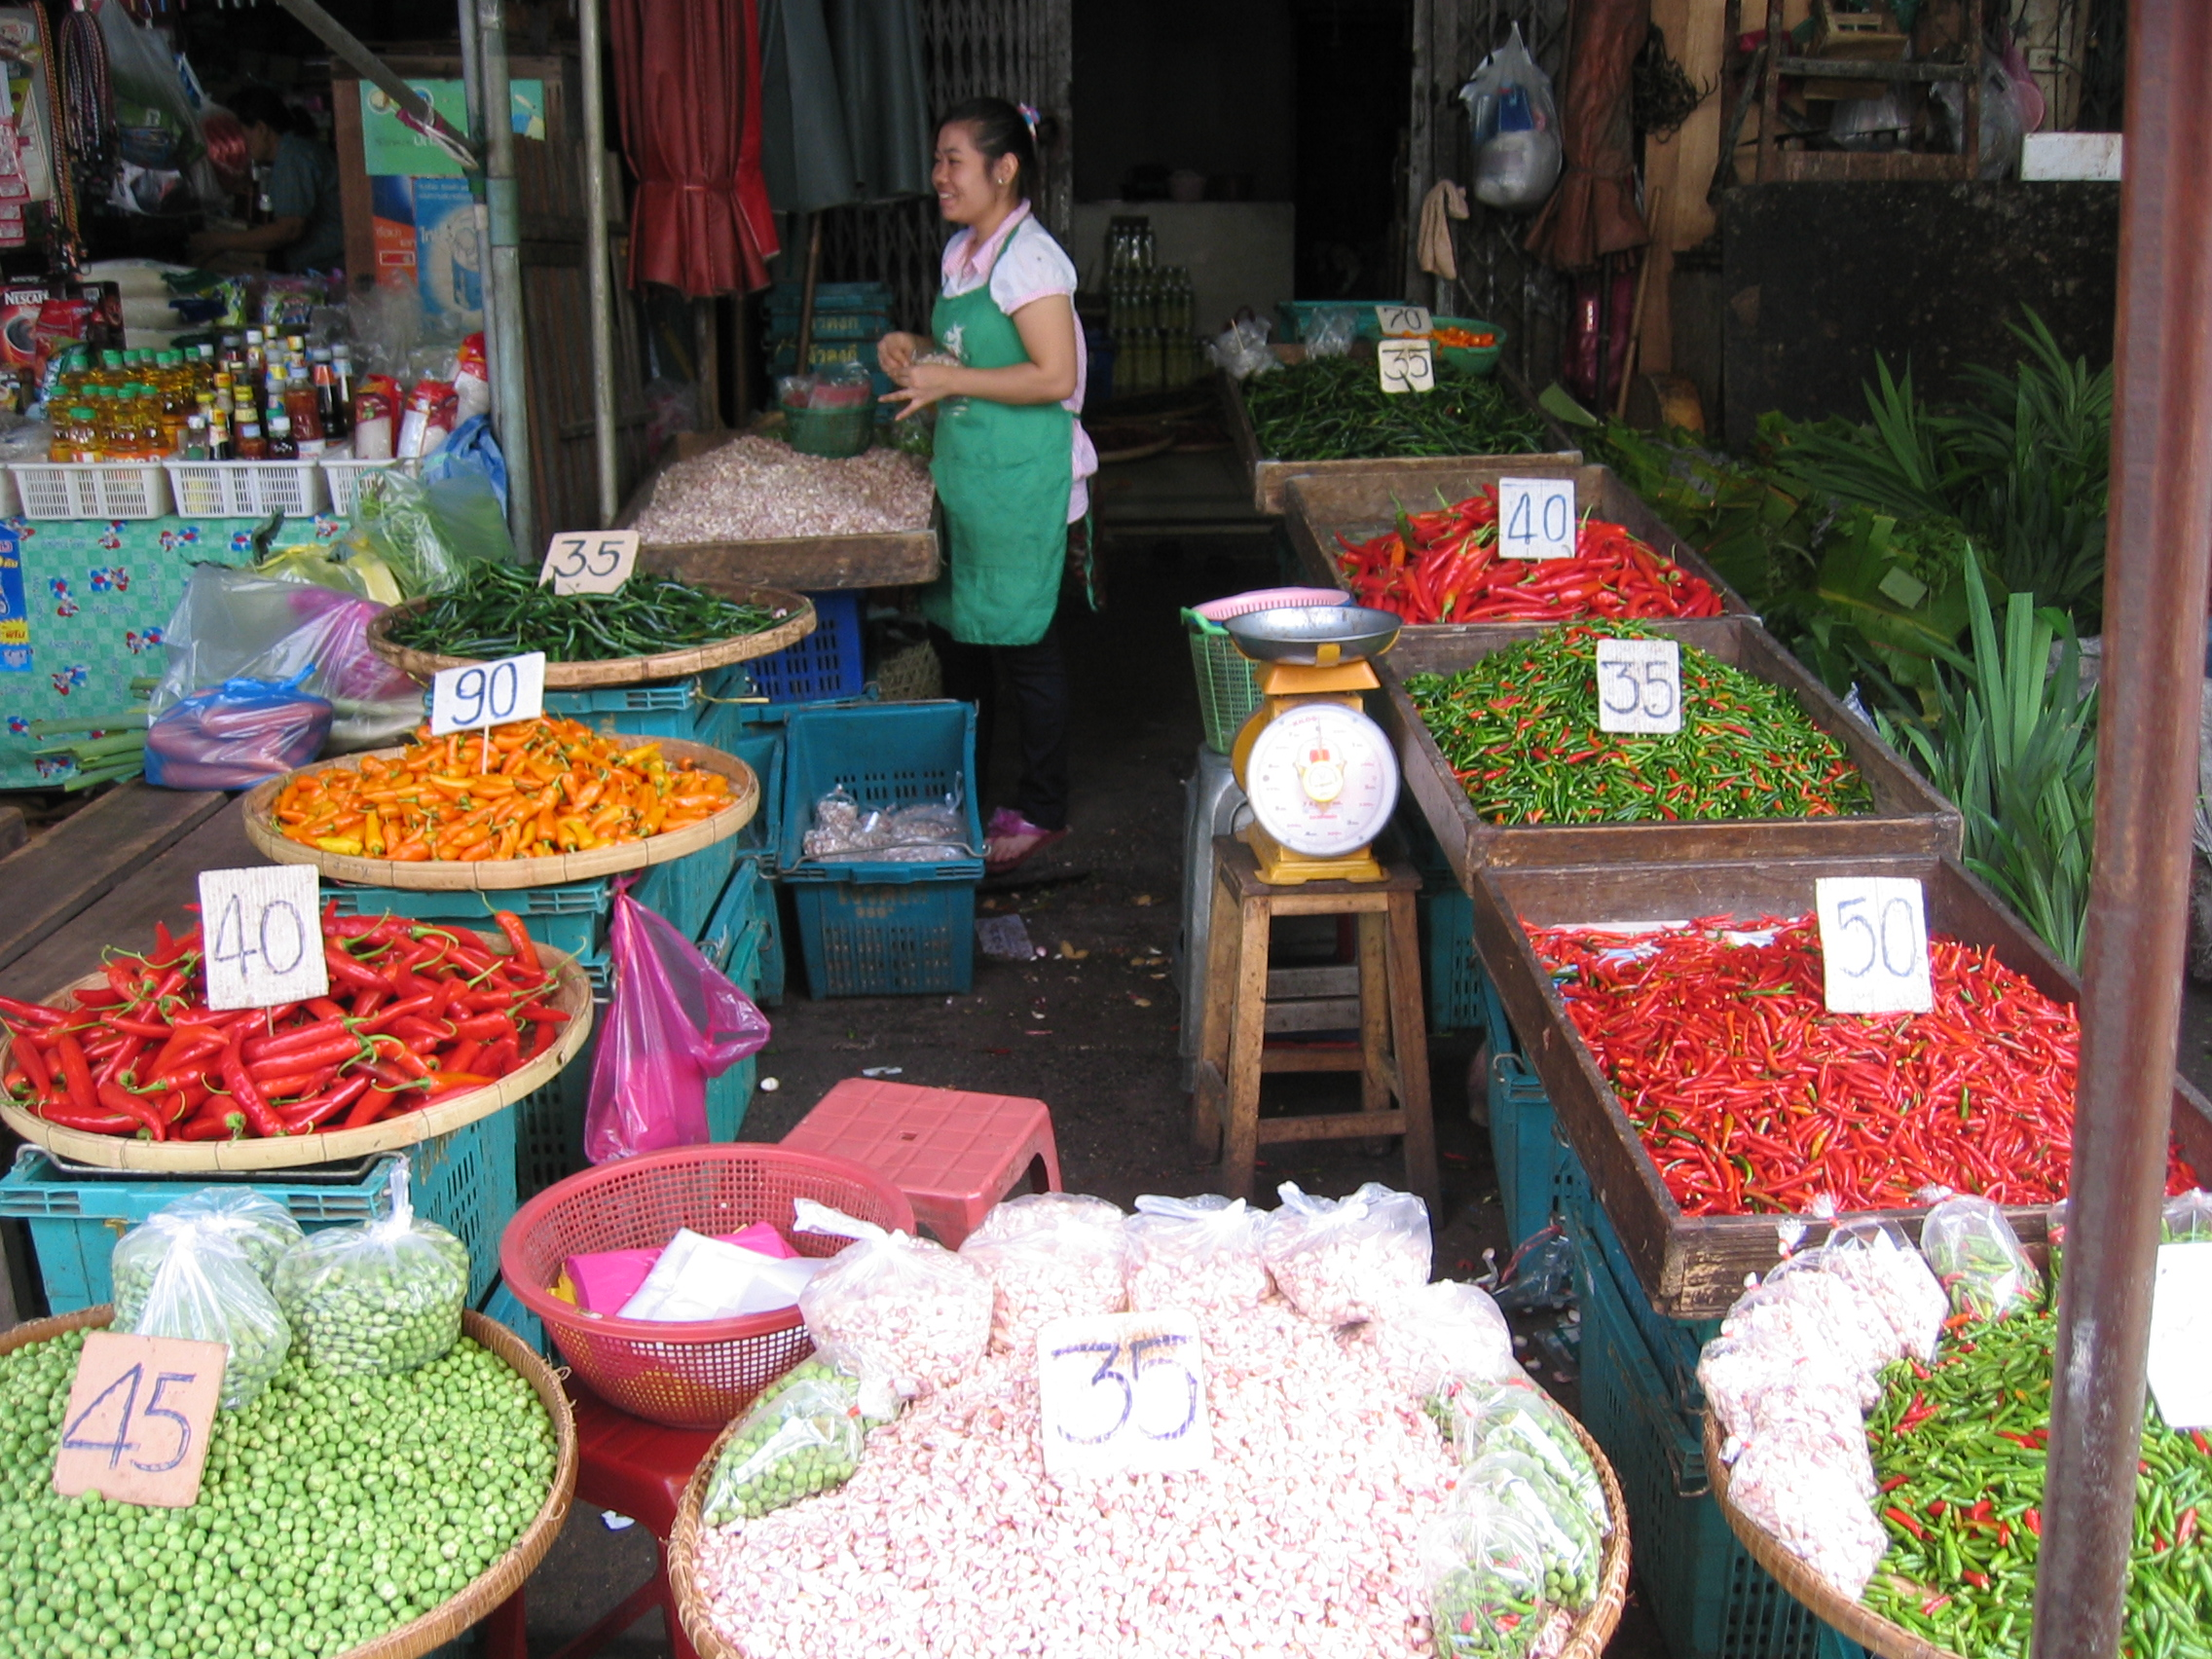
\includegraphics[width=5cm]{articles/Bangkok/1384.jpg}
%Un marché
\smallbreak

\smallbreak
\hspace*{-0.65cm}
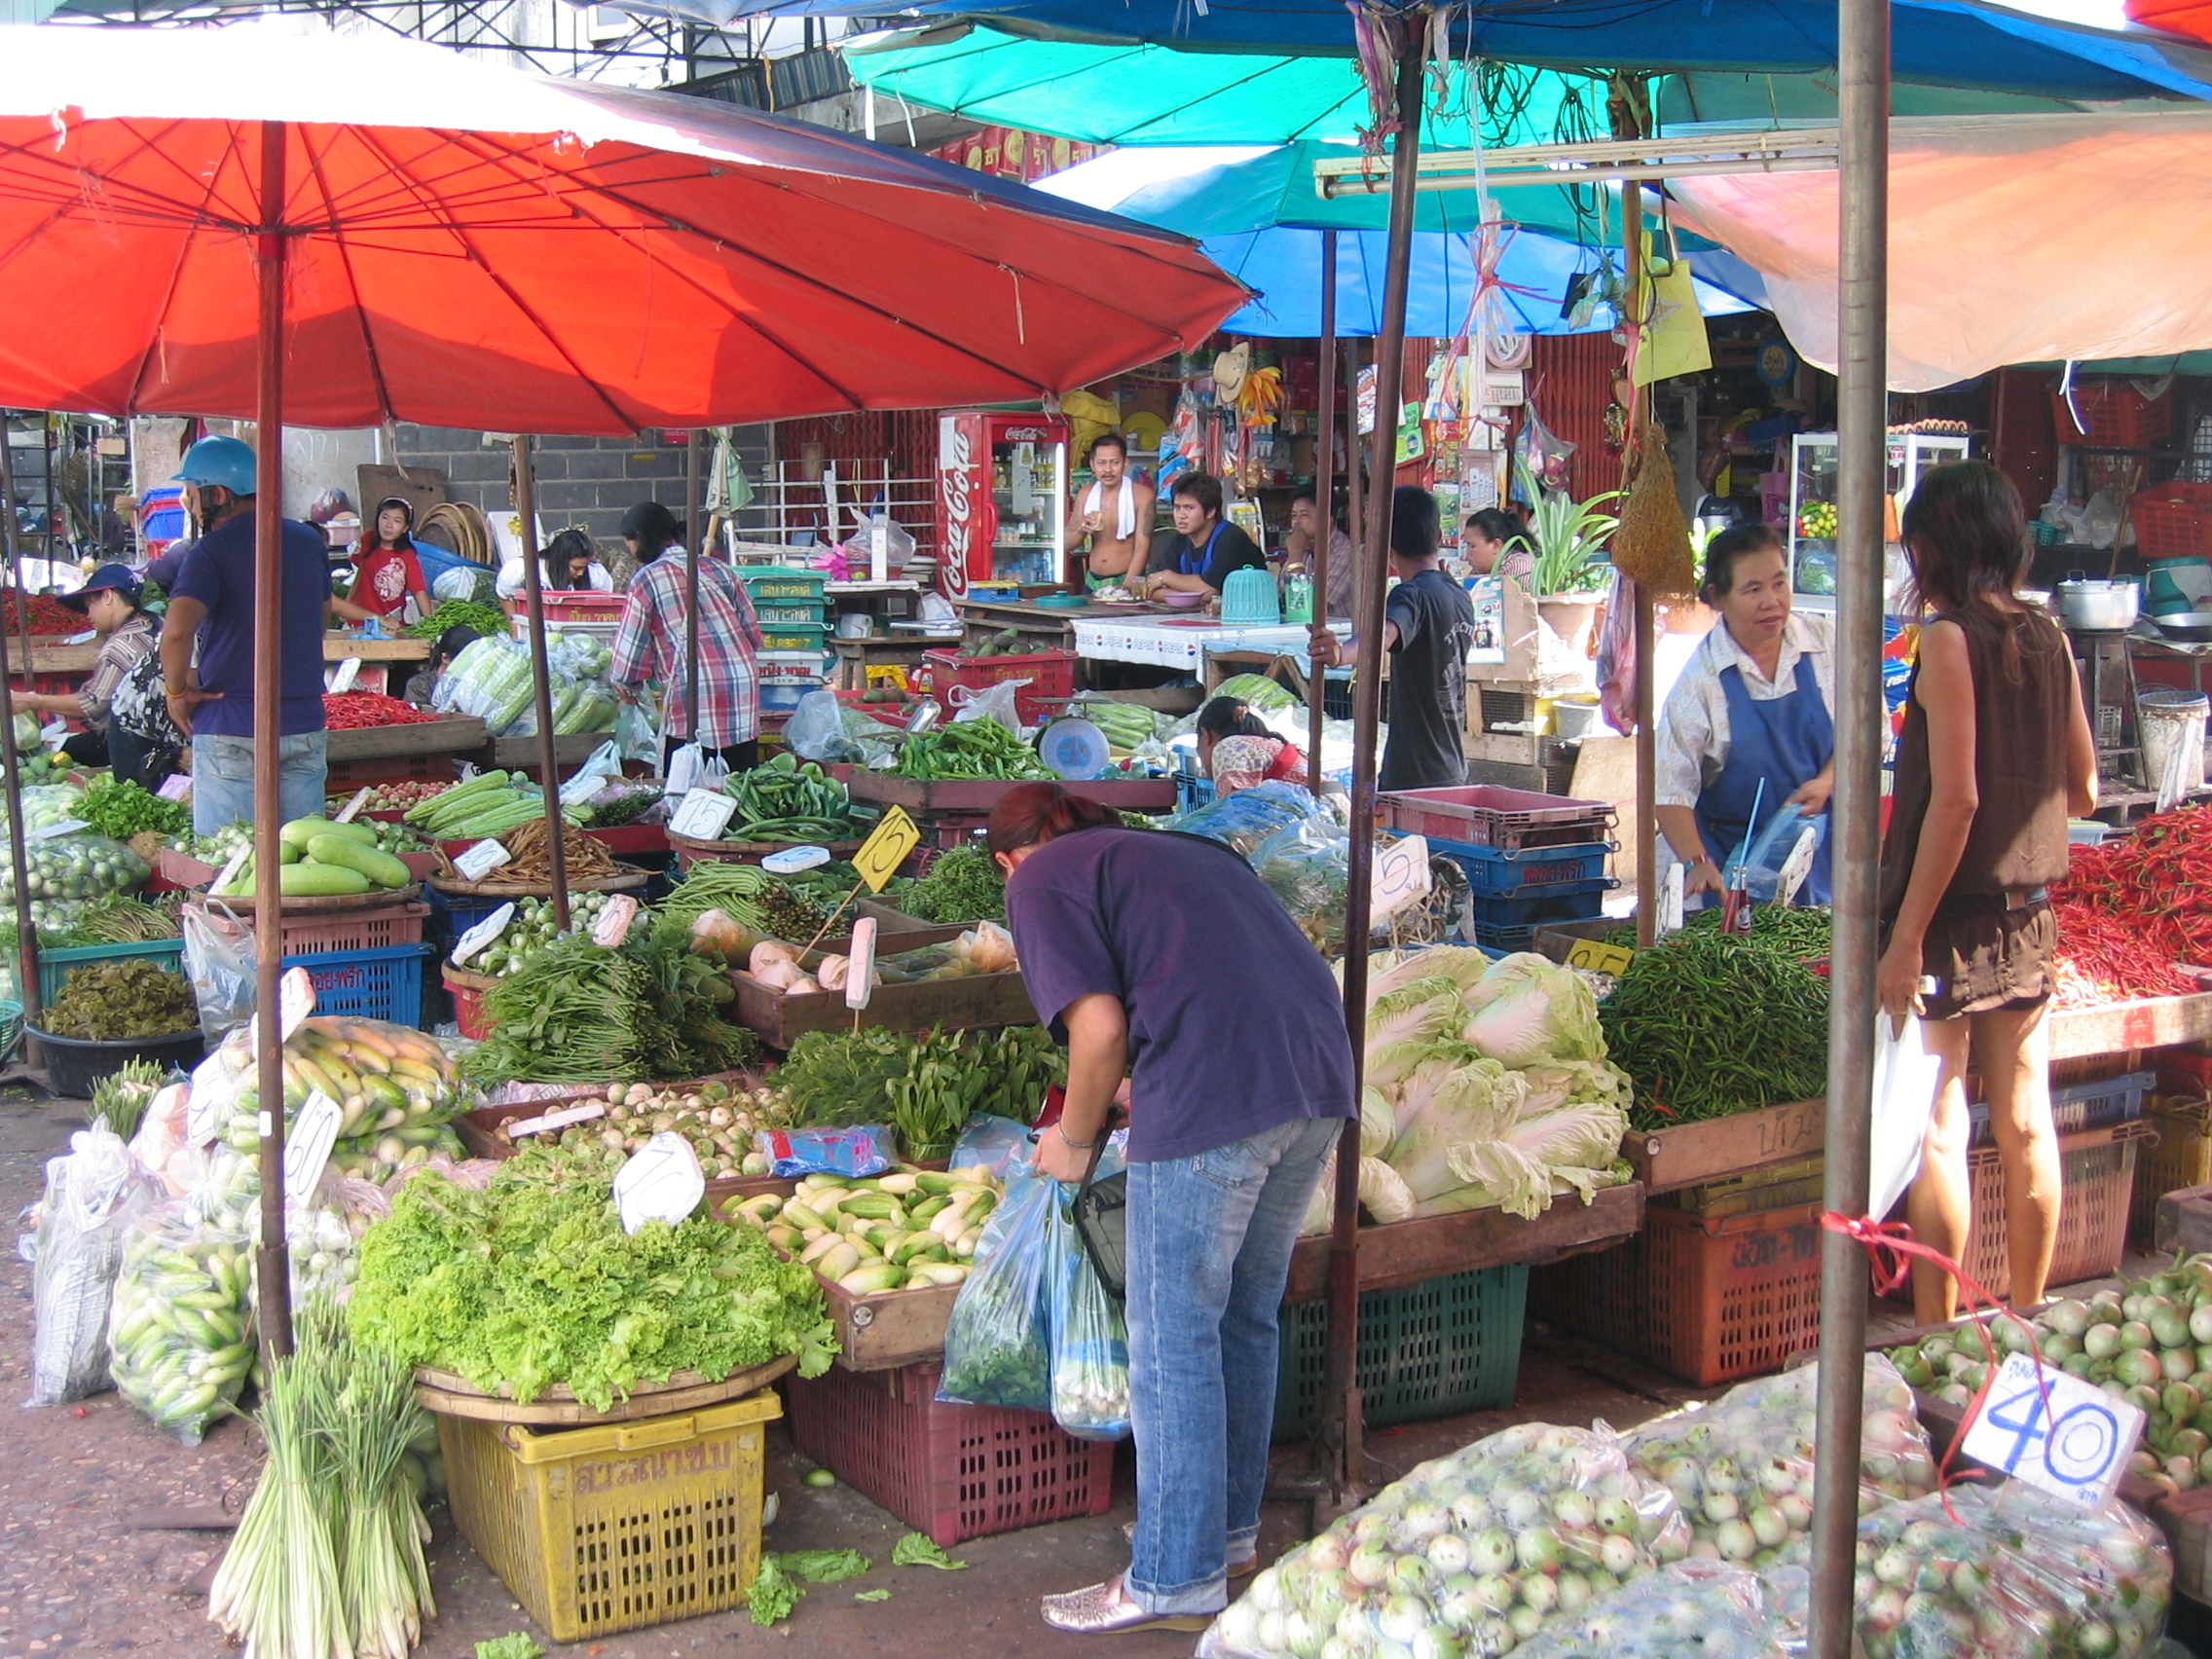
\includegraphics[width=5cm]{articles/Bangkok/1387.jpg}
%Une autre photo du marché
\smallbreak

%<div><object width="640" height="505"><param name="movie" value="http://www.dailymotion.com/swf/x5r4b7&related=1"></param><param name="allowFullScreen" value="true"></param><param name="allowScriptAccess" value="always"></param><embed src="http://www.dailymotion.com/swf/x5r4b7&related=1" type="application/x-shockwave-flash" width="640" height="505" allowFullScreen="true" allowScriptAccess="always"></embed></object></div>

Je ne vous dis pas au revoir ici, j'attaque directement l'article suivant sur Kanchanaburi.

\end{multicols}

\bigskip
\textbf{\textsc{Commentaires}}

\medskip
Titou a écrit le 15 juin 2008 :
\begin{displayquote}
Ehehe encore de jolies photos mon petit Dud !
En ce qui concerne le coulage des bonzes\dots je dirai que bizarrement le cerveau arrive a lire des mot qui ne sont pas forcément complets\dots mais je t'apprendrai ! il faut un R :) Content de te savoir en vie et en pleine forme. Profites a fond car ici c'est la misère\dots
Fais gaffe a toi et a plus.
Biz mon pote
\end{displayquote}

\vfill

